\subsection{Decision making in a bureaucracy\label{sec:decision-making}}


Occasionally events unfold without decisions being made. This might be because the decision makers are not informed, or there is an intentional neglect.

A \gls{simple decision} has one correct or beneficial choice and one or more wrong or harmful choices. The work of decision making is to gather information that identifies which is the correct or beneficial choice and select that option.

Best case scenario is one person making a well-informed simple decision that has immediate consequence and the consequence is to the decision maker. Example from elementary formal education: arithmetic math problems, multiple choice quizzes, spelling tests, memorization tests. 

A complex decision may have many choices, and there are might not be a best option. Then a \href{https://en.wikipedia.org/wiki/Pareto_front}{Pareto frontier} might exist where trade-offs can be made. 

As an example of a complex decision made by one person with immediate consequence and direct relevance to the decision maker, suppose you want to purchase a car. You car about only two aspects: fuel efficiency and cost. 

\begin{figure}[ht]
    \centering
    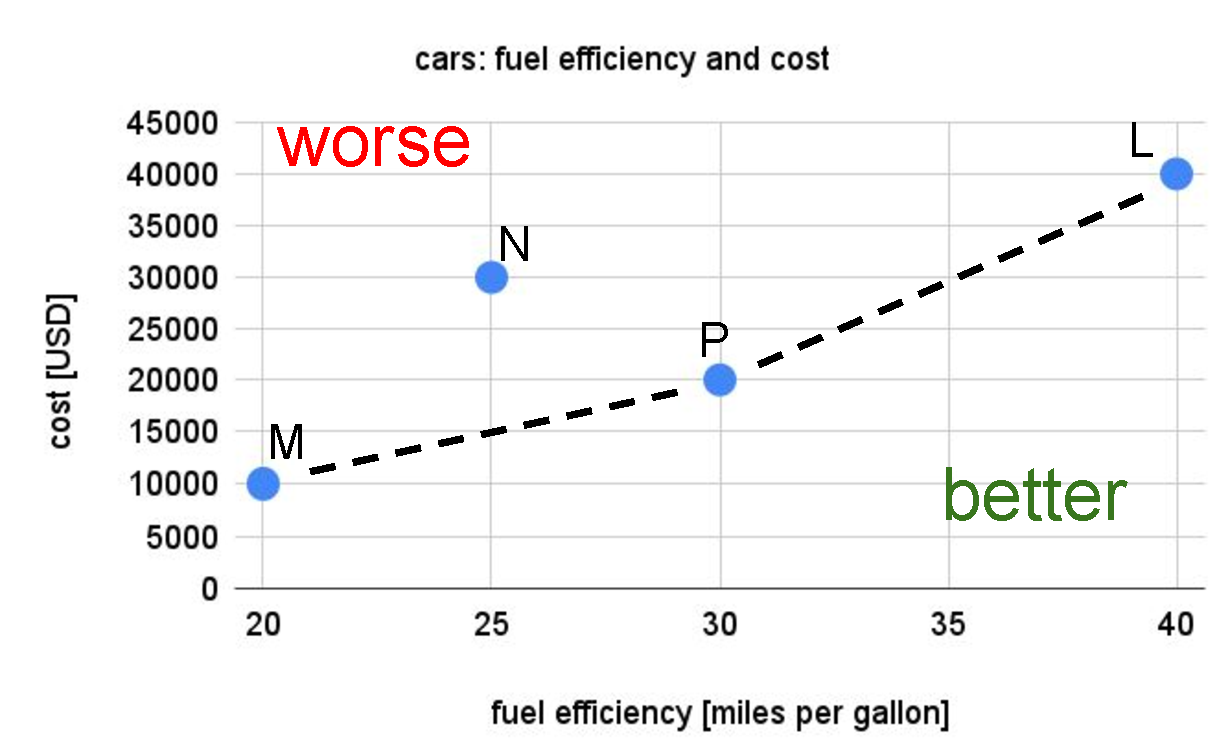
\includegraphics[width=1\textwidth]{images/pareto_frontier_car_options.pdf}
    \caption{Four cars, L, M, N, and P. Goal is to spend less money and get better fuel efficiency. Choices not on the frontier should be avoided, but that doesn't yield a single result.}
    \label{fig:pareto_frontier_cars}
\end{figure}

A common pareto frontier in generic decision making is the trade-off between speed, accuracy, and cost. 

Pareto frontier analysis works well when there are many options relative to the number of variables being optimized for. Does not account for relative importance of different variables.

The assessment does not work as well when there are few choices relative to the number of variables. For example, suppose there are 10 choices of car and I want high fuel efficiency, high cargo capacity, maximum number of passengers, stylish, low cost, low maintenance, good durability, and high resale value. might need to assign weights to each of these factors. 

A typical decision is ill-informed, has diffuse consequences, delayed impact, and does not affect the decision maker. 

Even afterwards a decision can be difficult to evaluate for correctness because there are multiple stakeholders.

In bureaucratic processes there is rarely a formal assessment of options. 
Decisions are rarely recorded. 



Process and policy\ref{sec:process}

One way to avoid the appearance of subjective decision making on policy is to frame the process as ``data driven." 
% https://graphthinking.blogspot.com/2018/06/data-driven-decisions-versus-data.html



% https://graphthinking.blogspot.com/2019/01/political-decisions-versus-science.html
A decision is political when the basis is historical relationships, maintenance or creation of a relationship, or to enable future relationships.
In contrast, a quantitative decision basis is based on measurements.


What appears from the outside as ``organizational inertia'' is internal delay of decision making and the delay of dissemination. 
Delay comes from
\begin{itemize}
    \item It takes time for each decision maker to gather information, arrive at a decision, modify processes, disseminate their selection, justify their selection. 
    \item forcing a continuous variable into a discrete set of choices. Typically the number of choices is small. Discrete choices for a continuous variable is a loss of effectiveness.
    % https://dynomight.net/teaching/
    \item processes designed to account for cheaters and people with malicious intent, whether that means a malicious bureaucrat or malicious subject. 
\item Analysis paralysis, due to {insufficient information, too much information, which framing is unclear}
\item When other people who are needed to carry out the action push back, either in disagreement or seeking clarification. The fact that the organization is not profit driven is important because the justification for the action isn't quantitatively obvious. Therefore there's a higher burden for communication.
\end{itemize}


Decision making by bureaucrats can be informal or formal, consensus-based or solo. 

Most decisions made by bureaucrats do not have hard deadlines. Instead, there are trade-offs in timing. Sooner is better, but delaying allows for more information gathering for a better informed decision.




Decision makers face options and have the goal of identifying a beneficial outcome (for which stakeholders?). The goal is to reduce uncertainty among options. Two ways to reduce uncertainty: gather more information (takes time), or push the decision down the chain (to people with narrower view). 

If a bureaucrat is going to rely on expert consultation, the decision maker needs to be confident the expert is not of straying outside their area of expertise. For example, I don't rely on a botanist with many published papers to tell me how to change the oil in my car. 

When getting input for a decision, is the expert providing a factual summary, a predictive assessment, or a value judgement? 

There are many ways to gather evidence. 
Role of measurement and modeling. 
Form an opinion, look for evidence to back the outcome.
Instead of measurement, most people rely on history (if they are aware of it), or what is best for their career, or how to accumulate more power, or what someone else says to do.  
